\chapter{Introduction and Market Overview}

\section{Background and Motivation}
Establishing a balanced supply-demand chain in the electricity system and taking precautionary steps to prevent grid blackouts or system damage is essential for the welfare of a country. A qualified authority can control the national grid with proper and timely actions.

\noindent\textbf{Reserve Market:}
Reserves are necessary to deal with the uncertainty inherent in electricity systems, such as forced outages and forecast errors. They are used to maintain the supply-demand balance at all times. These reserves can be provided by power plants, renewable generation units, storage units or flexible loads. System operators procure reserves well before the moment of delivery and activate them in real-time when needed to deal with imbalances.


\section{Electricity Market}
The electricity market refers to the framework where electricity is traded as a commodity, involving various transactions in long-term and short-term marketplaces. Electricity generation, transmission, distribution and retailing are managed by market regulators and actors through the day-ahead market, the intra-day market and balancing markets. This enables stakeholders to manage electricity supply, demand and costs effectively. A standard architecture is designed to ensure the efficient allocation of resources, promote competition to verify the robustness of a system, and provide incentives for investment in generation and infrastructure.

The concept of a market requires powerful authorities to investigate demand, develop a sustainable plan for seamless supply, distribute responsibilities to different actors and set laws for synchronisation across Europe. This requires a strong coordination chain among power producers, power demand actors, market operators, system operators, traders, BRPs, flexibility aggregators and consumers. Each of these actors contributes to the overall functioning of the electricity market and maintains a long-term plan to ensure stability in business.
\begin{figure}[htbp]
    \centering
    \IfFileExists{electricity_market.png}{%
        \includegraphics[width=0.8\textwidth]{electricity_market.png}%
    }{%
        \IfFileExists{images/electricity_market.png}{%
            \includegraphics[width=0.8\textwidth]{images/electricity_market.png}
        }{%
            \fbox{\parbox{0.75\textwidth}{\centering
            Image placeholder: add \texttt{electricity\_market.png} either beside \texttt{main.tex} or inside an \texttt{images/} folder.}}
        }%
    }
    \caption{Overview of electricity market actors and interactions}
    \label{fig:electricity_market}
\end{figure}


Some of the market actors are described below:

\noindent 1. \textbf{Power Producers and Portfolios:} A resilient electricity market relies on a diverse mix of generation technologies to ensure system stability and facilitate the large-scale integration of variable renewable energy. Producers optimise their presence based on the technical characteristics and marginal costs of their specific assets.
The primary types of power producers include:
\begin{itemize}
    \item Conventional Units: This category includes baseload and dispatchable providers such as coal, natural gas and nuclear plants, along with Combined Heat and Power (CHP) units, which provide the necessary inertia and reliability to the grid.
    \item Renewable Energy Sources: Decarbonisation efforts have led to a significant increase in renewable energy sources such as wind, solar, hydroelectric and biomass. These sources are variable and intermittent, requiring careful management and integration into the grid to maintain stability.
    \item Portfolio Owners: This group includes sophisticated entities managing a strategic mix of conventional and renewable assets, often distributed across the transmission network to hedge against localised risks.
\end{itemize}

\noindent 2. \textbf{Power Demands:} Participation as a power demand actor has become an active element of the grid and is a strategic tool for making this process flexible and balanced. By responding to price signals, consumption-side actors contribute to flattening demand peaks, which reduces system volatility and enhances grid stability. The main types of power demand actors include:
\begin{itemize}
    \item Large Consumers: This group includes major industrial plants that participate in the wholesale market as a primary means of managing high energy intensity and offering demand-response flexibility.
    \item Retailers: Retailers act as intermediate market actors or traders who purchase electricity at scale from the wholesale market. They build their business model on reselling this energy to a broad base of small-scale consumers, including households and small businesses.
\end{itemize}

\noindent 3. \textbf{Market Operator and Regulator:} This function is referred to as market governance and covers market transparency, maximisation of social welfare, and non-profit and neutral oversight. It is required to establish strong governance and a level playing field for all market participants. When these actors are viewed in a broader perspective:
\begin{itemize}
    \item Market Operator: This sub-group focuses on the financial administration of the market. They receive all bids and offers, execute the linear optimisation and disseminate market prices, volumes and winners. Some popular market operators include EPEX SPOT and Nord Pool.
    \item Regulator: Regulators form another sub-group; they monitor market performance for both short-term and long-term planning, enforce policies to prevent market manipulation, and ensure that the market operates to a standard that promotes competition, ensures reliability and protects consumer security.
\end{itemize}

\noindent 4. \textbf{System Operator:} A major coordination role is performed by system operators to maintain real-time supply security and system stability as a physical necessity that transcends financial contracts. System operators are the ``air traffic controllers'' of the grid, ensuring that the laws of physics are respected across different voltage levels.
    \begin{itemize}
    \item Transmission System Operator (TSO): The TSO is a key player in the electricity market, responsible for managing the high-voltage, meshed transmission grid. TSOs primarily stabilise the whole system and secure the supply chain. In Finland, Fingrid manages the transmission system and operates the balancing market. At a continental level, ENTSO-E is the association of European TSOs.
    \item Distribution System Operator (DSO): The DSO manages low- and mid-voltage radial grids that deliver power to end-users. A specific task for a DSO is the continuous monitoring of transformer loading to prevent local infrastructure failure. DSOs are responsible for ensuring reliable grid operation, integrating renewable energy, upgrading networks, investing in smart grid technologies, fostering consumer engagement and facilitating collaboration with local energy companies.

    For safe grid operation, TSO--DSO coordination is essential. The TSO balances the overall system while the DSO manages local congestion and grid integrity.
\end{itemize}

\noindent 5. \textbf{Specialised Market Participants and Emerging Actors:} The increasing penetration of renewables necessitates specialised roles to manage imbalances and provide the flexibility required for a modern grid.
    \begin{itemize}
        \item Balance Responsible Parties (BRPs): A market participant that is financially responsible for ensuring that the same amount of electricity is injected into the national grid as is withdrawn at the connection points for which the participant has balance responsibility.
        \item Flexibility Aggregators: These actors cluster smaller, distributed resources such as residential batteries to participate in wholesale markets as a single, significant block.
        \item Traders: Market participants who operate under two different types of trading policies. One is physical trading, where they have a direct impact on the physical flow of electricity, such as through battery assets. The other is financial trading, where they engage in contracts to buy and sell reserves in different markets without directly affecting the physical flow of electricity. Traders often utilise futures markets for long-term protection against price inflation, with contract durations of up to 6 years.
    \end{itemize}


\section{Types of Electricity Markets}
These market actors operate across three electricity market types: the Capacity Market, the Energy Market and the Ancillary Service Market. The purpose and working principle of each market are described below:

\noindent 1. \textbf{Capacity Market:} A capacity market is a mechanism in the electricity sector that ensures there will be enough power generation available to meet future demand. Power generators receive incentives for being able to produce a fixed amount of electricity within an allocated time and remain ready to supply power when needed, especially during peak demand. Capacity markets typically use forward auctions in the short-term (within a few hours or days) or long-term (a year ahead), where power providers commit to resource availability. Winners receive payments in exchange for the obligation of future capacity delivery. The unit of the delivered resource is measured in megawatts (MW).

\noindent 2. \textbf{Energy Market:} The energy market focuses on the trading of electricity as a commodity, where prices are determined by actual electricity production and consumption over time. The unit is measured in megawatt-hours (MWh). It allows participants to buy and sell electricity based on their needs and preferences. Generators earn energy payments for the electricity they actually deliver to the grid. The energy market operates across various timeframes, including day-ahead, intra-day and real-time markets (also known as the balancing market), allowing participants to adjust their positions based on changing conditions, forecasts and uncertainty in asset availability.

        \noindent 2.1. \textit{Day-ahead market:} The day-ahead market, also known as the spot market, allows participants to buy and sell electricity for delivery on the following day. The decision is made one day before the actual delivery, based on forecasts of supply and demand. Prices are determined through a competitive bidding process for a fixed time span, and the market operator announces the selected capacity providers within a short time. This market helps to ensure that there is sufficient capacity available to meet the expected demand for the next day and allows participants to plan their operations accordingly.

        \noindent 2.2. \textit{Intra-day market:} The intra-day market provides eligible participants with a second opportunity to adjust their positions in real-time as conditions change throughout the day. A timeframe is defined that begins just after the announcement of the day-ahead market results and continues until a predefined time limit before actual delivery the following day.

        \noindent 2.3. \textit{Balancing Market:} The balancing market is used to manage imbalances between supply and demand in real-time, ensuring that the grid remains stable and reliable.

        Each of these markets plays a crucial role in ensuring the efficient operation of the electricity system and facilitating the integration of renewable energy sources. The electricity market is a complex and dynamic system that requires careful management and regulation to ensure its efficient functioning and to meet the evolving needs of consumers and producers. The capacity market, energy market and ancillary service market work together to ensure sufficient generation capacity, efficient trading of electricity and reliable support services to maintain the stability of the power grid.

\noindent 3. \textbf{Ancillary Services:} The ancillary service market is responsible for providing support services that help maintain the stability and reliability of the power grid. These services include frequency regulation, voltage control and reserve power. The ancillary service market is crucial for ensuring the smooth operation of the electricity system and maintaining the balance between supply and demand in real-time.


\begin{figure}[htbp]
    \centering
    \IfFileExists{electricity_market_type.png}{%
        
\includegraphics[width=0.8\textwidth]{electricity_market_type.png}%
    }{%
        \IfFileExists{images/electricity_market_type.png}{%
            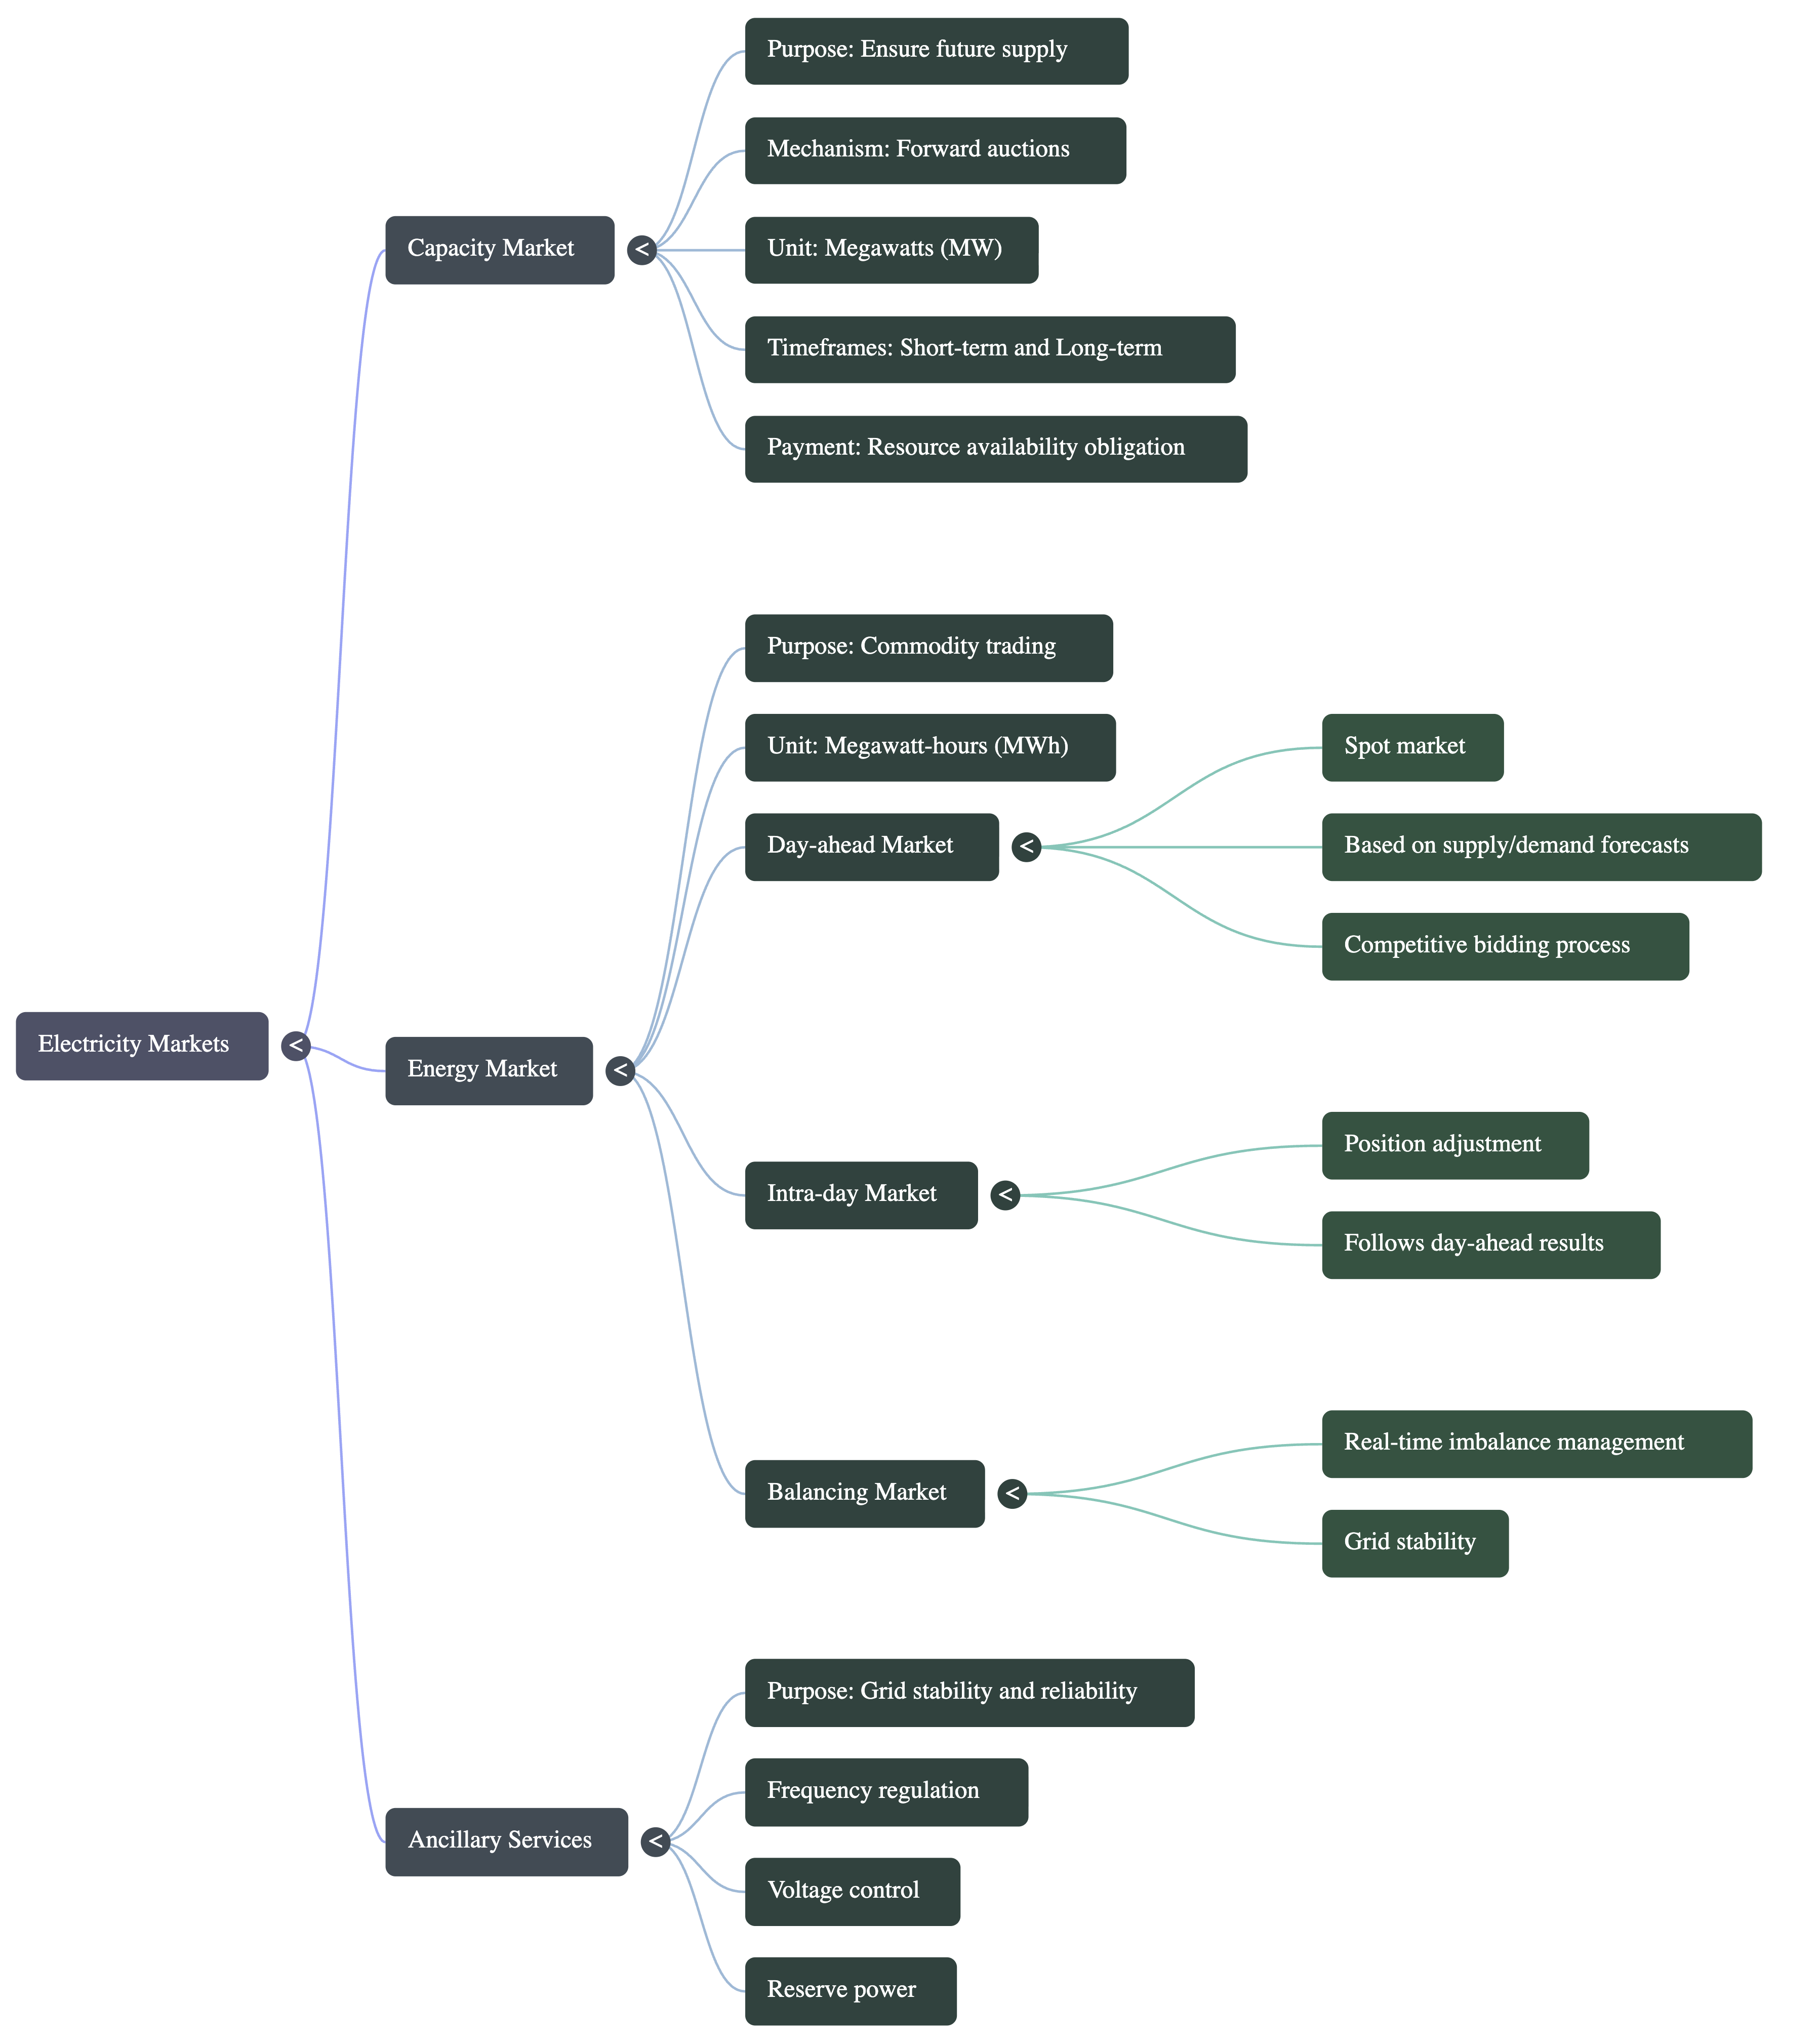
\includegraphics[width=0.8\textwidth]{images/electricity_market_type.png}
        }{%
            \fbox{\parbox{0.75\textwidth}{\centering
            Image placeholder: add \texttt{electricity\_market\_type.png} either beside \texttt{main.tex} or inside an \texttt{images/} folder.}}
        }%
    }
    \caption{Architecture of different electricity market types and their purposes}
    \label{fig:electricity_market_type}
\end{figure}

\section{Ancillary Services}
Ancillary services play a crucial role as a system safety net when the balancing market needs emergency support to stabilise the grid and safely operate the power system. These services are categorised into three major types:

\noindent 1. \textbf{Frequency-supporting services:} This category maintains the balance between power production and consumption instantaneously at the 50~Hz system frequency. Since frequency imbalance can cause serious issues such as equipment damage or grid blackout within a short time, it requires an active market to provide real-time support. Compared to other categories, frequency-supporting services are utilised more extensively due to the increased penetration of renewable energy. Therefore, maintaining system frequency within acceptable limits is crucial for the reliable operation of the power grid. Different products have significantly different technical requirements. There are several popular services traded across two main geographic regions: central Europe and the Nordics.

The main services in all European countries are:
    \begin{itemize}
        \item Frequency Containment Reserves (FCR)
        \item Automatic Frequency Restoration Reserves (aFRR)
        \item Manual Frequency Restoration Reserves (mFRR)
    \end{itemize}

    \noindent 1.1. \textit{Frequency Containment Reserves (FCR):} FCR, also known as primary control reserves, are activated automatically and within seconds to contain frequency deviations caused by sudden imbalances between supply and demand. They help to stabilise the system frequency by providing an immediate response to frequency changes. However, Nordic countries and the eastern part of Denmark cannot rely on general FCR because these areas have a low-inertia system. The shift from traditional synchronous generation (such as nuclear and large thermal plants) to inverter-based renewable energy resources (such as wind, solar and hydro) has significantly reduced the rotating mass and inertia in the Nordic power system. In a low-inertia system, an imbalance causes grid frequency to drop much faster than in a high-inertia system. Additionally, renewable energy is highly variable and production never remains within a limited range. A robust system is therefore required to handle different scenarios separately and reliably. This high penetration of renewable energy with high variability in the Nordic region increases the need for sophisticated frequency control strategies and faster response times to maintain grid stability. As a result, the Nordics have introduced special services called FCR-N, FCR-D and FFR. A separate market has been designed to prevent high-speed disturbance reserves from being exhausted by minor daily variations.

        \noindent 1.1.1. \textit{FCR-N:} This reserve is also known as FCR for normal operation. It is a symmetric product used to manage frequent, minor fluctuations within the normal frequency range of 49.9~Hz to 50.1~Hz. Service providers must be capable of providing both upward and downward regulation.

        \noindent 1.1.2. \textit{FCR-D:} FCR-D, or FCR for disturbance, is an asymmetric product activated during significant disturbances when the frequency deviation crosses the normal range. This reserve is further divided into two categories: FCR-D up-regulation for frequency drops in the range of 49.5~Hz to 49.9~Hz, and FCR-D down-regulation for frequency rises in the range of 50.1~Hz to 50.5~Hz. This gives service providers more precise control over frequency stabilisation in specific circumstances.

        \noindent 1.1.3. \textit{FFR:} Fast Frequency Reserve is a special reserve designed for rapid response to handle unpredictable low-inertia events. FFR acts as fast-acting support within one second to prevent further frequency drop.

    \noindent 1.2. \textit{Automatic Frequency Restoration Reserves (aFRR):} aFRR, also known as secondary control reserves, are activated automatically within a few minutes to restore the system frequency to its nominal value after a disturbance. They help to maintain the balance between supply and demand over a longer time frame compared to FCR. Similar equipment setup is required for aFRR as for FCR.

    \noindent 1.3. \textit{Manual Frequency Restoration Reserves (mFRR):} mFRR, also known as tertiary control reserves, are activated manually by the system operator within a specified time frame (usually 15 minutes) to restore the system frequency and manage larger imbalances. They provide additional support to the system and help to ensure the overall reliability of the power grid. No special equipment setup is required for mFRR.


\noindent 2. \textbf{Voltage-supporting services:} In this category, voltage is stabilised by controlling reactive power supply. This is often a local problem resolved through specific contracts rather than an active market.

\noindent 3. \textbf{Black-start services:} This category covers services that revive a power system after a blackout and take all necessary steps to restart the system.
\begin{figure}[htbp]
    \centering
    \IfFileExists{ancillary_services_architecture.png}{%
        
\includegraphics[width=0.8\textwidth]{ancillary_services_architecture.png}%
    }{%
        \IfFileExists{images/ancillary_services_architecture.png}{%
            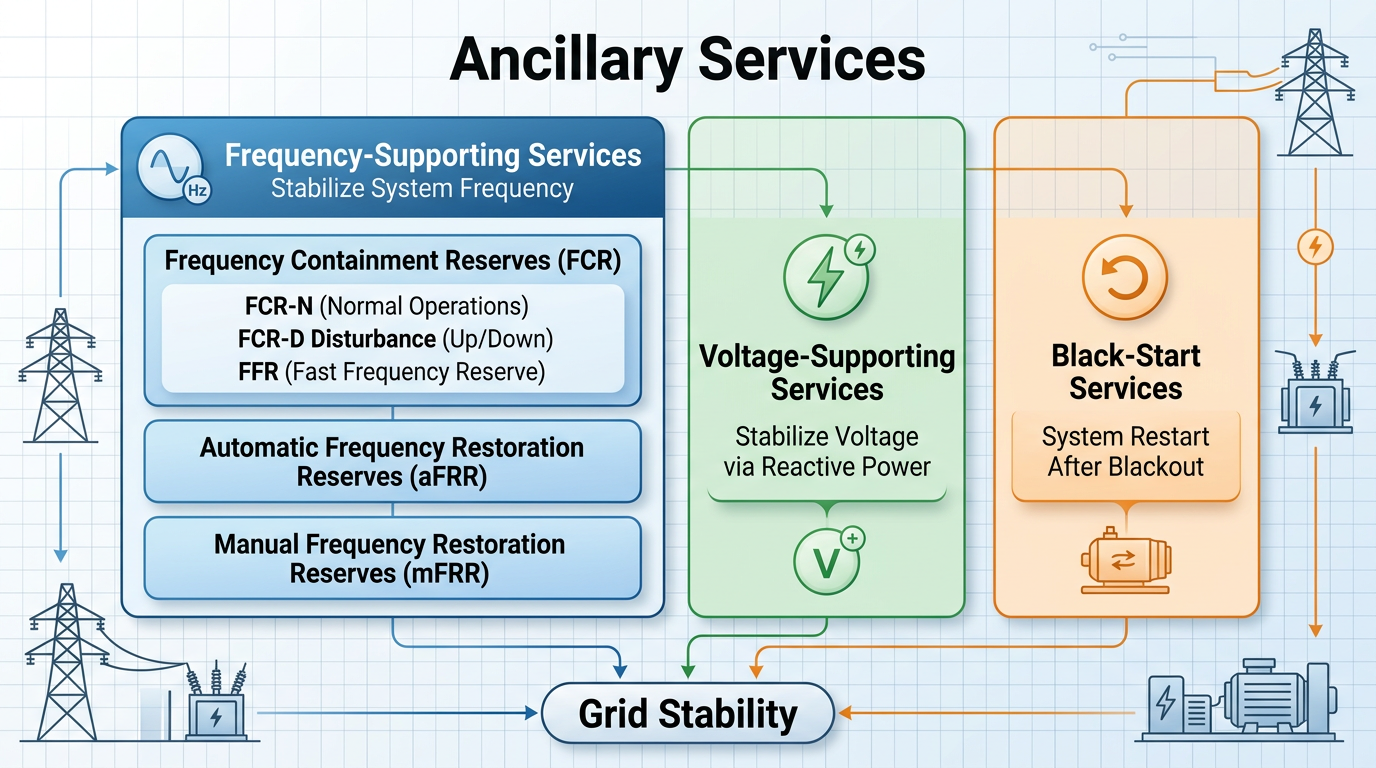
\includegraphics[width=0.8\textwidth]{images/ancillary_services_architecture.png}
        }{%
            \fbox{\parbox{0.75\textwidth}{\centering
            Image placeholder: add \texttt{electricity\_market\_type.png} either beside \texttt{main.tex} or inside an \texttt{images/} folder.}}
        }%
    }
    \caption{Architecture of ancillary services by type and purpose}
    \label{fig:ancillary_services_architecture}
\end{figure}


\section{Auctioning of Ancillary Services}
An auction is a competitive process where qualified market participants submit bids to provide ancillary services using the energy resources available to them. Market operators or regulators use auctions to contract a specific volume or capacity at the lowest price. This auctioning process does not offer a fixed price; rather, it provides scope for market participants to determine prices intelligently through competition. The competition ensures transparency, promotes cost-effectiveness and provides an overview of market dynamics for future business. Auction winners sign a short- or long-term agreement and guarantee a revenue stream that benefits both parties. The sequential stages of the energy auctioning process are as follows:
    \begin{itemize}
        \item Announcement and Design: This step is conducted by the market operator to announce the auction, outlining rules, opportunities, prequalification requirements and the timeline.
        \item Prequalification: Interested BSPs, aggregators or traders undergo prequalification tests following predefined requirements to demonstrate their technical capabilities and financial and legal eligibility to provide the service. After successful tests, they submit documentation on the overall process and performance with supporting technical illustrations. This is the approval stage for bidding.
        \item Bid Submission: Approved participants submit their bids on a fixed date with detailed information about the price per megawatt.
        \item Bid Evaluation: Bids are assessed by the market operator based on predefined criteria. Different countries have variations in evaluation methods, and the strategy to win a bid in one country does not necessarily apply to another.
        \item Awarding and Contracting: One or multiple bidders can be selected based on evaluation results. Winners sign a contract with the market operator for a specific period, with confirmation of payments either for capacity reservation or real-time energy delivery, depending on the market type and contract terms.
        \item Reserve Delivery and Settlement: The final stage is the delivery of contracted services. Participants must provide the agreed-upon ancillary services during the contract period. The market operator monitors performance and settles payments based on contract terms. In the case of capacity reserves, payment is made for the availability of the service regardless of whether it is activated. In contrast, real-time energy delivery is compensated based on the actual amount of energy delivered when the service is activated. In most countries, penalties are imposed if the participant fails to deliver the contracted service or delays delivery.
    \end{itemize}
\begin{figure}[htbp]
    \centering
    \IfFileExists{auction.png}{%
        
\includegraphics[width=0.8\textwidth]{auction.png}%
    }{%
        \IfFileExists{images/auction.png}{%
            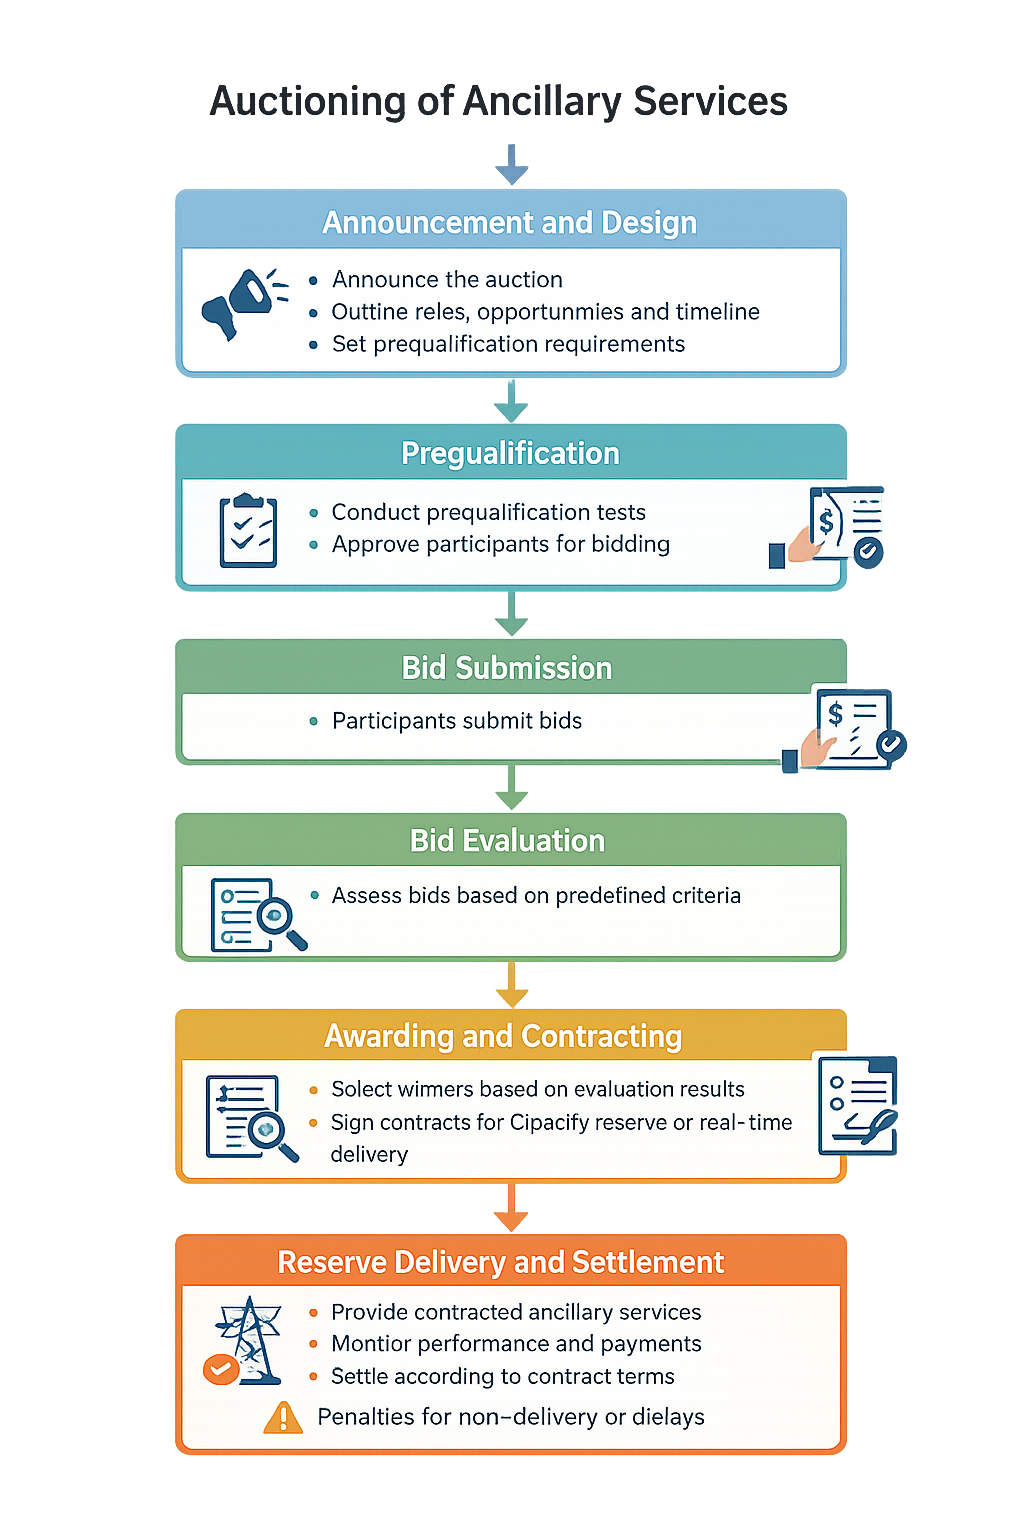
\includegraphics[width=0.8\textwidth]{images/auction.png}
        }{%
            \fbox{\parbox{0.75\textwidth}{\centering
            Image placeholder: add \texttt{auction.png} either beside \texttt{main.tex} or inside an \texttt{images/} folder.}}
        }%
    }
    \caption{Different stages of auctioning process for ancillary services}
    \label{fig:auction}
\end{figure}


\section{Emergence of Prequalification Test}
To manage these ancillary services effectively, system operators procure them through dedicated markets. These markets are regulated by TSOs, BSPs and BRPs to allow efficient allocation of resources and ensure that the necessary reserves are available when needed. TSOs disclose strategies and controls to bring every BSP onto a common platform, which is called the reserve market. The reserve markets for FCR, aFRR and mFRR are designed to facilitate the procurement process and enable market participants to supply contracted services under governance. Participation in these markets requires compliance with specific technical and operational requirements, including the installation of appropriate equipment to enable remote monitoring and control. With proper evidence and agreement, participants become Balance Service Providers (BSPs) for a fixed period. Therefore, demonstrating both technical strength and safety is a key prerequisite for passing the prequalification test before entering the reserve market.

Prequalification is the process that ensures market participants meet the necessary technical, communication and error-handling requirements to provide ancillary services. This process typically involves testing and verification of the participant's capabilities, including their ability to respond to frequency deviations within predefined time windows and to provide uninterrupted service. It verifies the robustness of signal capture and the appropriateness of the actions taken by the BSP to handle moderate to critical situations that could otherwise cause the national grid to collapse. In this process, participants need to demonstrate performance under various scenarios. For FCR, the key parameters include minimum and maximum capacity, activation time limits, meter accuracy, central asset requirements, non-LER duration and error margin, among others. For aFRR, significant parameters include activation time, capacity, sampling time, non-LER duration and error margin.

There is a notable difference between FCR and aFRR prequalification test requirements. Nevertheless, most European countries share similarities in terms of requirements such as activation time, capacity, non-LER duration and frequency meter accuracy. ENTSO-E and the SOGL exercise a strong influence on both the FCR and aFRR markets. Regarding activation time, the initial activation following a frequency deviation must begin within 2 seconds, 50\% of the reserve must be delivered within 15 seconds, and the full reserve must be delivered within 30 seconds as committed during the auction. Participants must fulfil a minimum capacity of 1~MW in all countries, though some require a maximum of 25~MW, which introduces an additional requirement to verify resource sustainability. This is referred to as the Limited Energy Reservoir (LER). If technical units are not capable of providing uninterrupted reserve supply over an extended period, the service provider must agree to extended requirements and setup measures to overcome the shortcomings. On the other hand, central asset, linearity, error margin and sampling time requirements appear relatively uniform across countries. However, not all TSOs provide clear instructions on these terms. For example, the central asset requirement concerns the frequency meter used to measure the current frequency of the grid. Each TSO instructs different rules for meter installation based on the overall grid system setup, electricity regulation, and supply and demand conditions, in order to extract accurate data. The limitations imposed on how TSOs validate results and the degree of flexibility allowed raise concerns among participants regarding the strengths and weaknesses of each TSO's process. In such cases, the service provider will choose to proceed with the TSO where the most data is available and requirements can be matched.


Some European countries are included in this study and are divided into three zones based on similarities in prequalification test requirements. Those zones are: Northern Europe, Central Europe and Southern Europe. In the Northern zone, countries such as Denmark and the Baltics are included. In the Central zone, countries such as Belgium, Germany, the Netherlands, Austria, Switzerland and several other nations are included. Finally, countries such as Spain, Italy and France are considered part of the Southern zone. The Northern zone follows rules and regulations similar to those of Finland. A thorough examination of the requirements for providing ancillary services clearly reveals that Finland has more similarities with the Northern zone. For instance, local asset requirements, tests, capacity thresholds and error margins are similar across these regions.


\section{Bidding}
Bidding is the first real communication with the TSO before the technical test. It is a process in which the TSO and interested parties participate to determine the price, capacity and penalties for the services. Bidding is a crucial step in the procurement of ancillary services, as it allows market participants to compete for contracts and ensures that the necessary reserves are procured at competitive prices. It also demonstrates the robustness of a system, its controller and its technical units in balancing sensitivity and reliability. Depending on the market, a date is fixed by the TSO and confirmed via email or other communication channels to willing participants. Bidders follow internal strategies or market trends to predict pricing and bid amounts. Some countries have shown balanced pricing and reduced losses when participants do not obtain their expected price. On the other hand, some countries can produce unexpected outcomes compared to predictions. The bidding process typically involves the submission of bids by market participants, which include details such as the price they are willing to accept for providing the service, the capacity they can offer and any penalties they are willing to accept for non-performance. The TSO evaluates the bids based on predefined criteria and selects the winning bids that best meet the system's needs while ensuring cost-effectiveness. The bidding process helps to ensure that there is sufficient competition in the market and that the necessary reserves are procured at reasonable prices, ultimately contributing to the reliability and stability of the power grid.

\clearpage
